\documentclass{article}
\usepackage{graphicx} % Required for inserting images
\usepackage{tcolorbox}
\usepackage{amsmath}

\title{Module 1}


\begin{document}

\section*{What is a database?}
A database is a collection of \textbf{data items} or facts that are stored systematically and permanently in a computer so that programs can consult it to answer questions. The answers to those questions are then processed to become \textbf{information} which can then be used to make decisions that may not be made with the data elements alone. Data items in a database differ from variables in a program since data items are intended to be permanent whereas program variables are discarded once the program terminates. Further, databases differ from an input file to a program (e.g. CSV) in that databases are more structured and allow for indexed access that is much faster than the sequential access often required by input files.

The facts may be structured in a number of ways, known as a \textbf{database model}, which is managed by a \textbf{database management system (DBMS)}, and queries using a query language.

Early DBMS (1960s) used a \textbf{hierarchical database model} or a \textbf{network database model}. During this time, query languages were very similar to programs. Many current DBMS use the \textbf{relational database model} which arrange facts into sets of values which satisfy logical predicates. SQL is the standard language and is declarative.

More recent 'NoSQL' systems use document-oriented models, key value stores or graph models, and have languages influence by relational languages.

Suppose we want more data in our database for each of our data items. Note that expanding the number of columns is not always wise as space consumption increases and the potential for lots of null values grows. May be better to link multiple tables together, which may prove to be easier to manage and keep consistent. For instance, when developing a calendar application, you may initially wish to have one table containing all events with details about the friend you will be going with and such. However, this a lot of information that may be difficult to maintain, unnecessary since we know that your phone has a list of contacts which are stored in a separate table. Can then just keep a table for events which links to your table of contacts. Linking does require some sort of unique ID matching between the tables and this is easy enough to manage using a third table that keeps track of which contact IDs map to which event IDs. Look below for an example: 

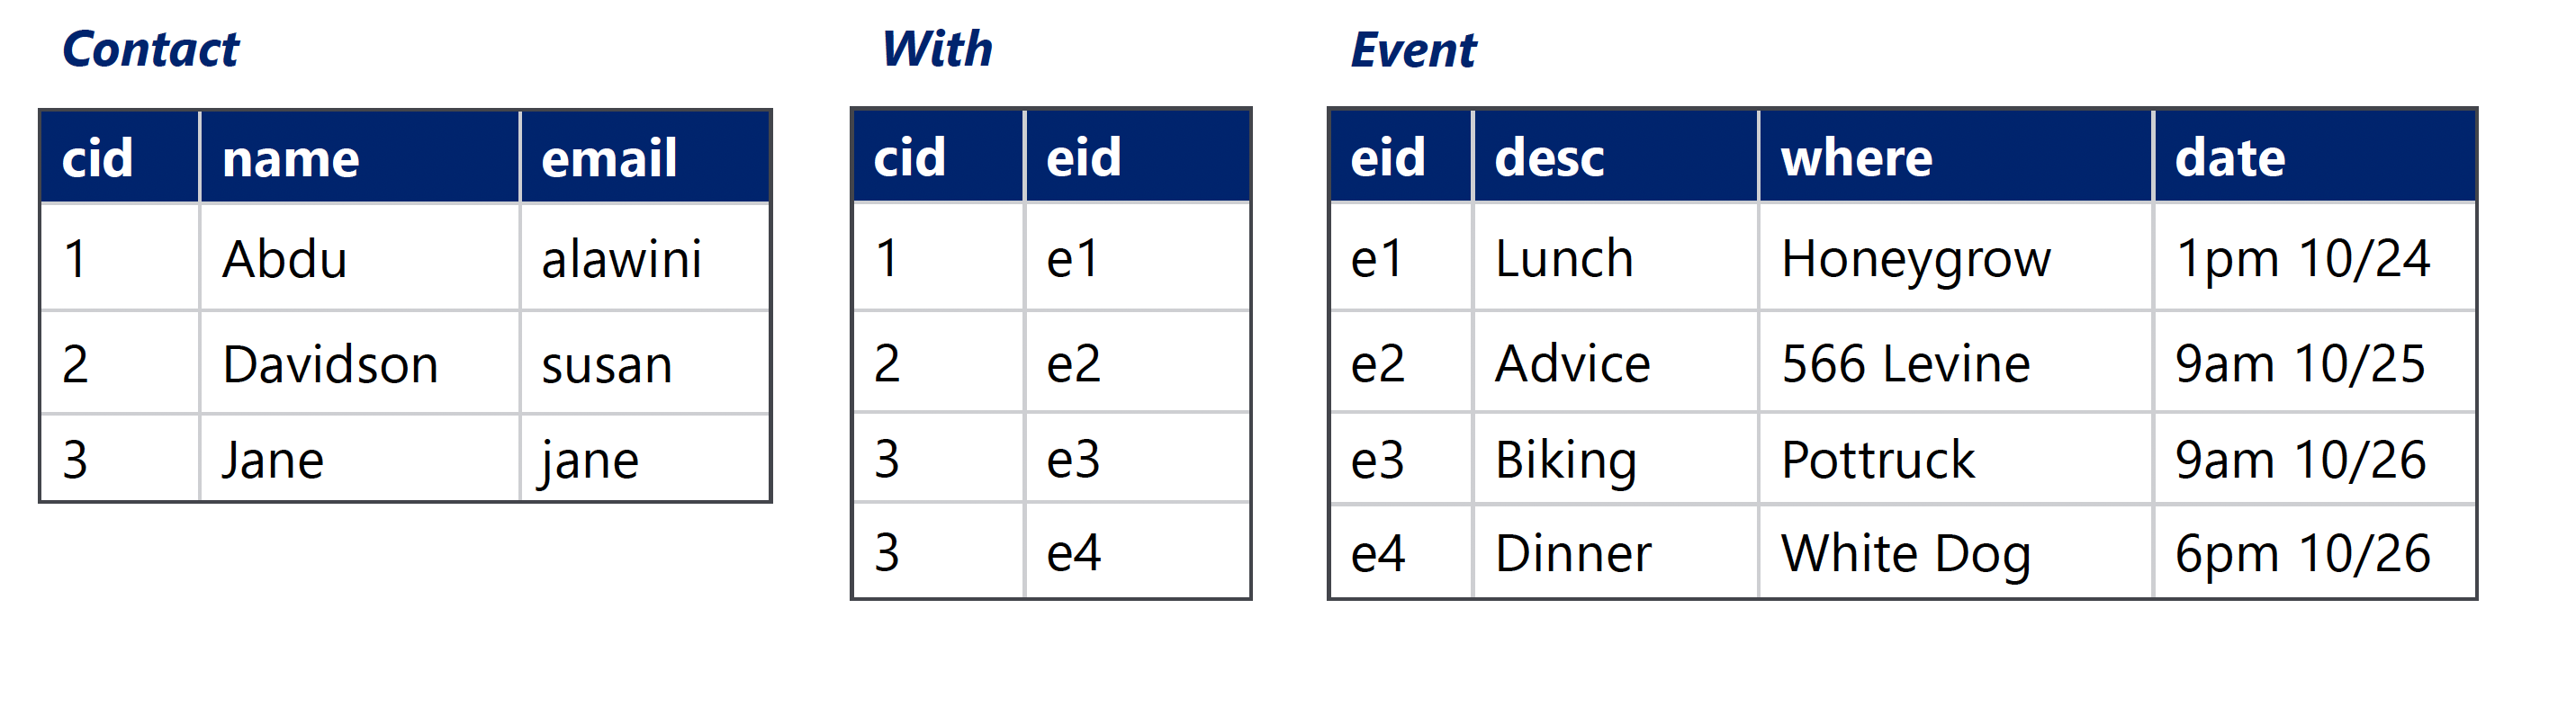
\includegraphics[width = 10cm]{assets/calendarExample.png}

Notice how similar this idea of 'linking' is to pointers in C/C++.

The data we've come across so far all have an implicit data model. Relevantly, the relational database model was the first model that is independent of its data structure and implementation. A \textbf{theory of normalization} guides you in designing relations. These same concepts have been adapted to form other data models such as object-oriented data models, XML, etc. We will focus mostly on the relational model and other models that 'borrow' ideas from it. 

\section*{What are the benefits of a DBMS?}
A database management system(DBMS) is a software package that is designed to store and manage databases. DBMS facilitate reliable storage and recovery of 100s of GBs of data. They further facilitate querying and updating via an interface or an API. Lastly, they provide support for concurrent users.

So why can't we code up our own DBMS?
\begin{itemize}
    \item Much simpler to use a DBMS specific to our purposes. Programmer does not need to understand complex details like indexes, sort orders, machine speeds, disk speeds, concurrency, etc. Instead, the user programs with a \textbf{logical model} in mind. Further, it allows the user to be \textbf{declarative} by querying with something like 'Give me all appointments on 10/28' instead of 'Loop over all Events and return those with a date of 10/28'.
    \item Surely it would not be too difficult to code up a DBMS for managing a small database of say, a 100 entries. However, the task becomes increasingly more challenging as the number of entries increases. So, we can say that a DBMS \textit{scales} very well.
    \item How do we ensure that concurrent access of the database does not cause issues, that data is kept consistent across all users, that the database remains reliable despite adverse events such as system crashes.
\end{itemize}
We begin our design of a database by formulating a logical model where we specify the model with tables and constraints. Following this, we need to do the 'physical' design -- the layout on disk, indexes, etc.

SQL is a declarative language and is often embedded into programming languages such as Java or JavaScript. SQL is based on restricted first-order logic expressions over relations. Basically, we're trying to specify what we want from some database tables using a set of logical expressions. Notice, this is not procedural, we are NOT telling the DBMS \textit{how} to find the data, we are just specifying \textit{what} data we need. The SQL query is then converted into a query plan and executed using the \textbf{query optimizer} and the \textbf{query execution engine}.

While we speak on the value of databases however, note that 80 percent of the world's data is not stored in a database. Examples of data not stored in a relational database management system (RDBMS) include scientific data, personal data, WWW and email, and logs - of searches, page accesses, traffic, etc. Some of this data is stored in something resembling a DBMS however. And data management is expanding to tackle these problems.

\section*{Relational Databases: Terminology}
The relational data model stems from insight by E.F. Codd in a breakthrough paper written in 1970 which asserted that we must separate the physical implementation from the logical (abstraction) and that we must model the data independently from how it will be used. The data must be described minimally and mathematically -- a relation is a set of tuples with attributes. And we must use standard mathematical (logical) operations over the data -- these being relational algebra or relational calculus. Took a number of years (1980s) for this approach to take hold, for commercial relational databases to appear. Lag can be explained by desire to do things in ways that were already established (inertia), people not wanting to write math formulas, not wanting to convert their data to tables, not believing this approach to be performant, and politics. 

Let us consider the below image containing a table (or relation) representing bank accounts. Recall that a relation is just a set of tuples with attributes.

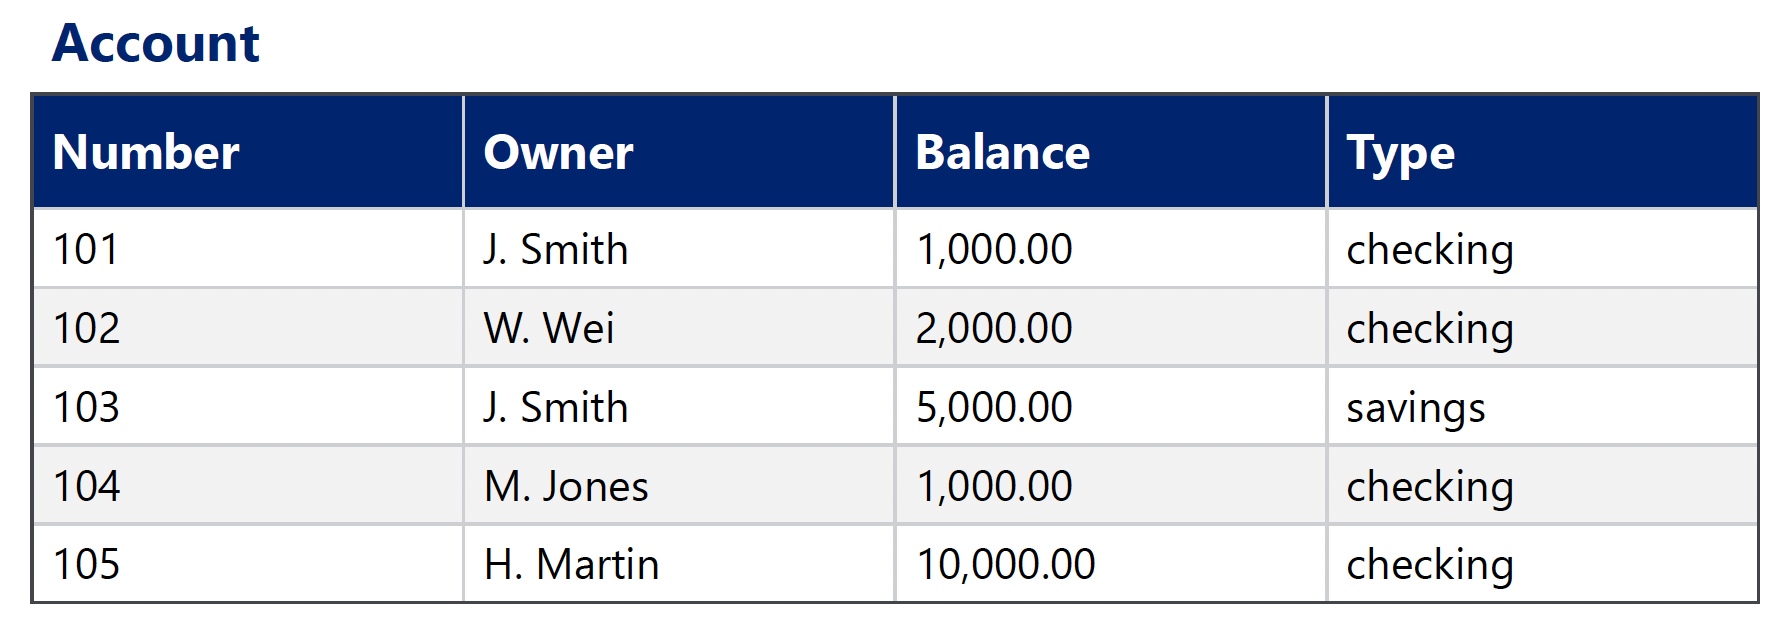
\includegraphics[width = 10cm]{assets/bankAccountsExample.png}

The name of the above table is \textit{Account}. The names of the \textbf{columns (attributes)} can be seen in the top row e.g. \textit{Number} or \textit{Owner}. The \textbf{schema} for the table sets the structure of the table and can be thought of as the definition of the table. This schema includes the various attributes of the table as well as the name of the table. Looking at the actual data in the table, each entry in the table is called a \textbf{row (or tuple)}. Sometimes an entry in the table is called a \textbf{record}. The actual set of all records in a table is called an \textbf{instance} of the table. The same table as above with one record deleted and two new records, for instance, would be considered another instance of the table. Similar to the schema, the \textbf{intension} of the table includes the name of the table and the set of attributes with their constraints. The \textbf{extension} of the table includes the set of all actual records. The \textbf{degree} or \textbf{arity} of a table is the number of columns and the above table has an arity of 4. The \textbf{cardinality} of a table, on the other hand, is the number of rows in the current instance, which for our example instance is 5.

Keep in mind that the relational model consists of tables(or relations) with attributes, called the schema which changes slowly over time. On the other hand, an instance of the table (so non-header rows) change quickly over time. The degree or arity of a table is the number of columns and the cardinality is the number of non-header rows. And a relational database consists of many, inter-related tables.

\section*{Relational Databases: Constraints}
We know that a database consists of one or more tables. Each table must have a key where the values are unique. Keys must consists of one or more columns per table. These keys allow us to uniquely identify data in a table and link it with corresponding data in other related tables. Now, how do we prevent nonexistent/incorrect keys from being added to tables? Well, we utilize the concept of \textbf{foreign keys} which map a key attribute in one table to a \textbf{primary key} attribute in another table representing the relationship between the tables where one table is referencing another table. Look at an example of this below:

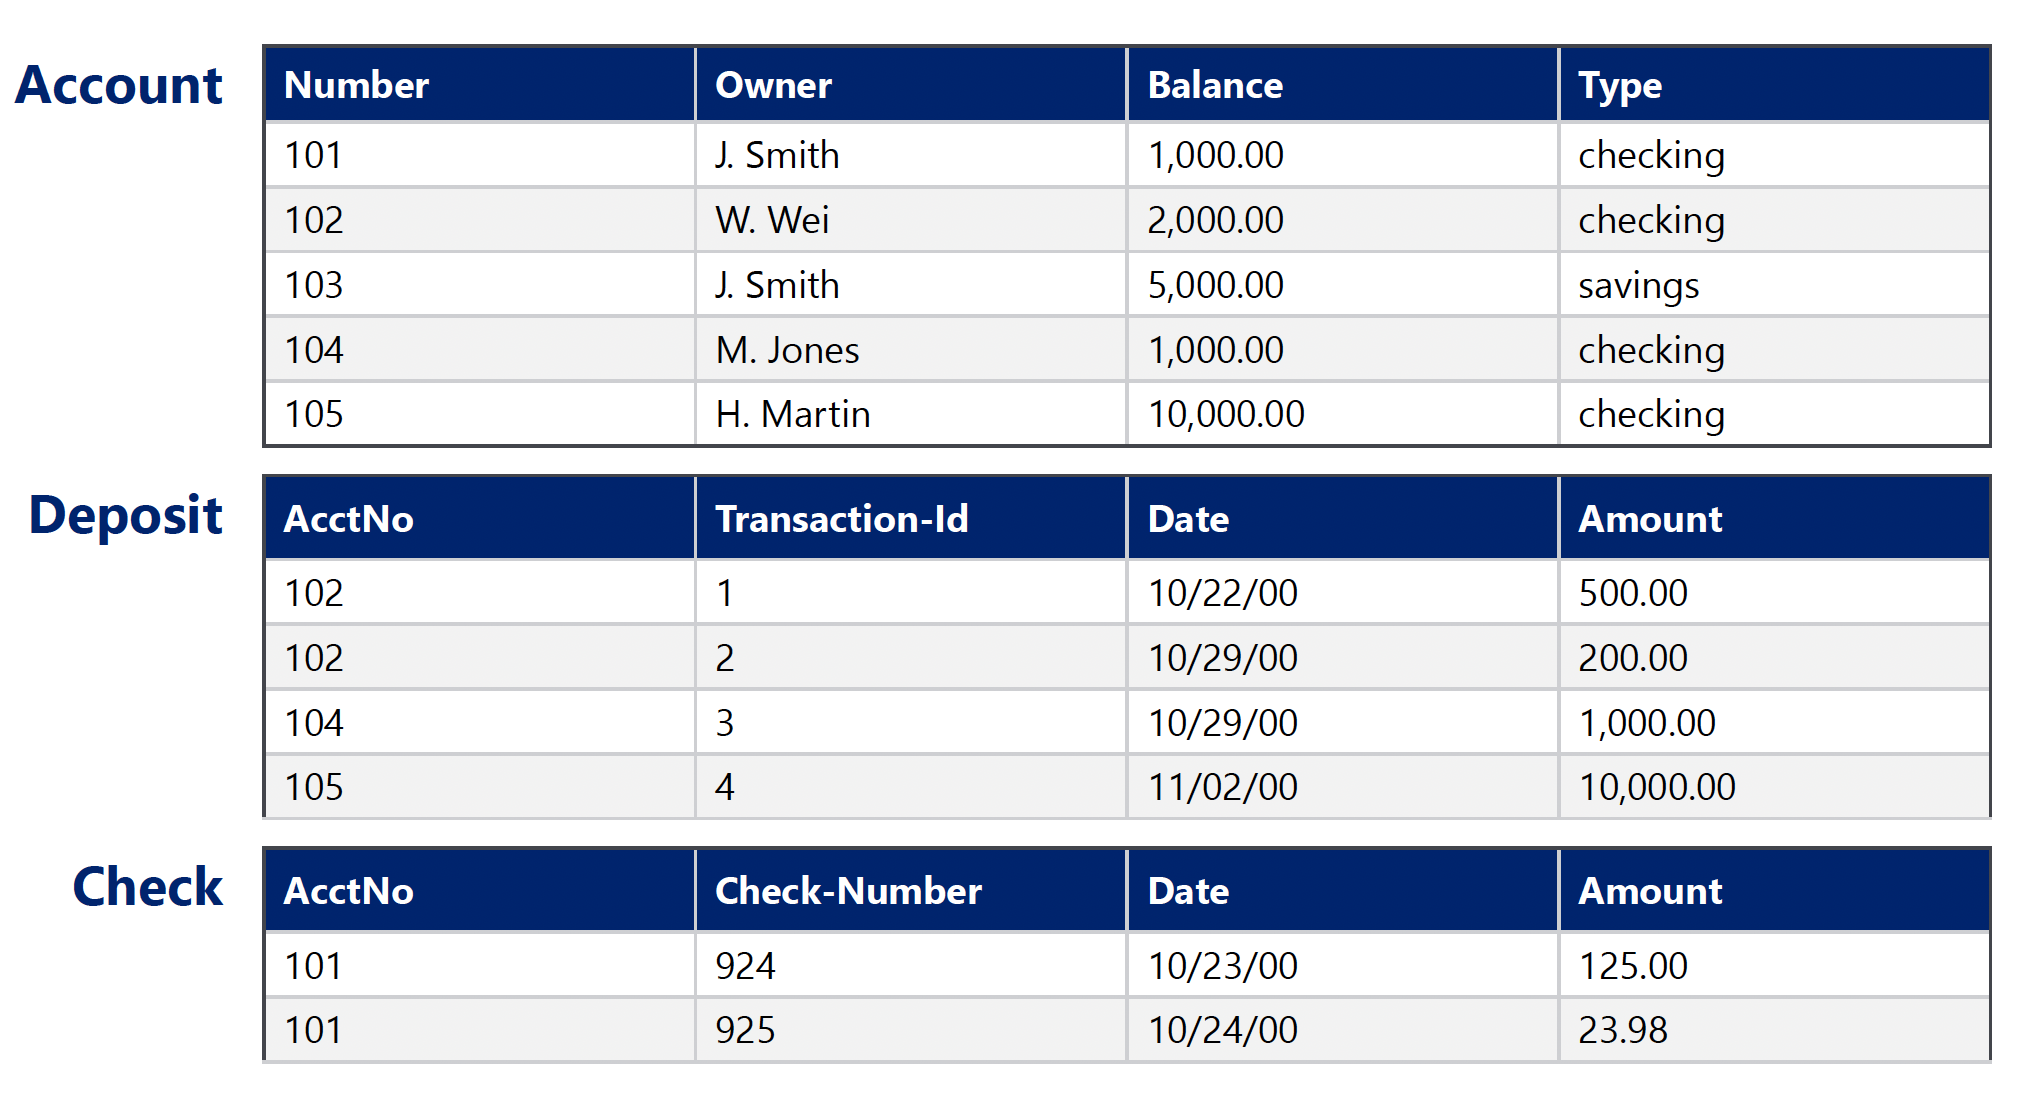
\includegraphics[width = 10cm]{assets/bankAccountsExample2.png}

\textit{AcctNo} in the \textit{Deposit} and \textit{Check} tables serve as foreign keys that reference \textit{Number} in the \textit{Account} table. This prevents incorrect records being added to a table that reference some nonexistent account number -- this constraint's enforcement facilitates \textbf{referential integrity}.

Keep in mind that keys and foreign keys are constraints-- semantic assertions -- about valid database instances. And multiple attributes may serve as the key for a table in some cases, such as when you have a table with columns listing date, salesperson, customer, and sale amount. Would not use sale amount as a key but could use a combination of date, salesperson, and customer as the key since none of those attributes must have unique values on their own. Furthermore, in many-to-many relationships, an additional 'all-key' table may need to be introduced, where the key consists of foreign keys to the original tables.

\section*{SQL Data Definition Language}
SQL is the standard language for relational data -- invented by folks at IBM. There have been a series of SQL standards and DBMS products vary in how much of the standard they support. Importantly, SQL can be separated into a \textbf{DML (data manipulation language} and a \textbf{DDL (Data Definition Language}. DML is based on relational algebra and calculus which we will discuss later. 

The DDL specifies the database schema. The tables, with a name for each table. The attributes for each table and the domain for each attribute. The key(s) for the table. And all foreign keys. Keep in mind that there \textit{can} be more than one key for a table. One is chosen as a primary key and the others are called 'alternate' keys and are indicated using the keyword \textbf{UNIQUE}.

Recall our previous bank accounts example. For every attribute in the \textit{account} table, the schema specifies allowable values e.g. \textit{Number} must be an integer, \textit{Owner} must be a 30-character string, \textit{Balance} must be money (DECIMAL(19,2)) where 19 is the number of integers and 2 is the number of decimal places, and \textit{type} must be 'checking' or 'savings'. Note that the set of allowable values for an attribute is called the domain of the attribute.

Look below to see how we specify this same schema in SQL DDL:

\begin{tcolorbox}
    \begin{verbatim}
    CREATE TABLE Account (
        number  INT,
        owner VARCHAR(30),
        balance DECIMAL(19, 2),
        type ENUM (`checking', `savings'),
        PRIMARY KEY (number) )

    CREATE TABLE Check  (
        acct_no INT,
        check_number INT,
        date DATE,
        amount DECIMAL(19, 2),
        PRIMARY KEY (acct_no, check_number),
        FOREIGN KEY acct_no REFERENCES Account (number) )
    \end{verbatim}
    
\end{tcolorbox}
Note how \textit{Check's} primary key consists of more than one attribute.

To insert rows into \textit{Account} and \textit{Check}, we no longer need DDL, we can just use the DML or data manipulation language which you can see in action below. Remember, DDL is just for \textit{defining} tables.

\begin{tcolorbox}
    \begin{verbatim}
        INSERT INTO Account
        VALUES      (101, `J. Smith', 10000, `checking'),
                    (102, `W. Wei', 2000, `checking'),
                    (103, `J. Smith', 5000, `savings');

        INSERT INTO Check
        VALUES      (101, `J. Smith', 10000, `checking'),
                    (102, `W. Wei', 2000, `checking'),
                    (103, `J. Smith', 5000, `savings');
        
    \end{verbatim}
\end{tcolorbox}

Note how the records for \textit{Check} must be added after those for \textit{Account} since we need to maintain referential integrity and the foreign keys in \textit{Check} reference the primary key in \textit{Account}.

\section*{Single Table Queries}
Let us take a look at the basic syntax of SQL
\begin{tcolorbox}
    \begin{verbatim}
        SELECT [DISTINCT] {list of attributes}
        FROM {list of relations}
        WHERE {conditions}
    \end{verbatim}
\end{tcolorbox}

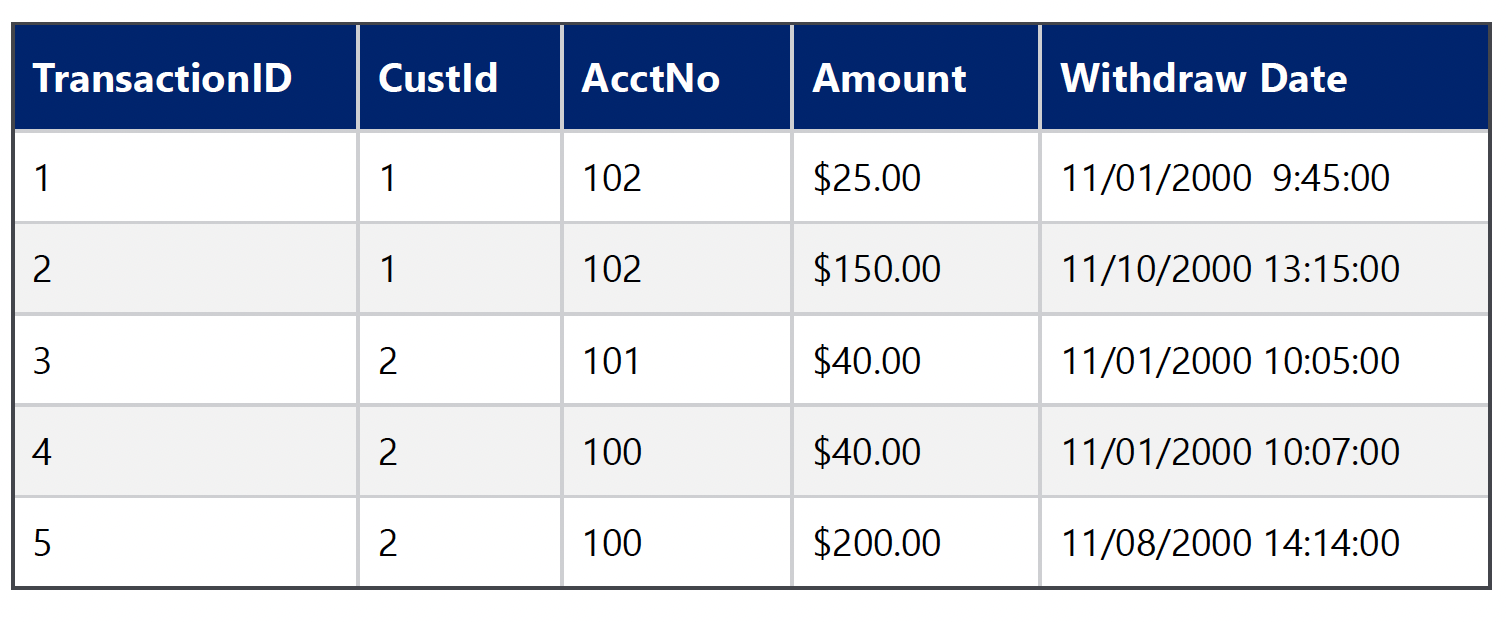
\includegraphics[width=10cm]{assets/ATMWithdrawalExample.png}

Now, how would we create a query to return the \textit{acctNo} and \textit{amount} attributes for amounts less than 50 dollars from the \textit{ATMWithdrawal} relation?

\begin{tcolorbox}
    \begin{verbatim}
        SELECT AcctNo, Amount
        FROM ATMWithdrawal
        WHERE Amount < 50;
    \end{verbatim}
\end{tcolorbox}
Note that the \textit{WHERE} clause is evaluated for each tuple in the relation.

Now, how would we get all attributes from the \textit{ATMWithdrawal} relation where \textit{TransactionId} is 3?

\begin{tcolorbox}
    \begin{verbatim}
        SELECT *
        FROM ATMWithdrawal
        WHERE TransactionId = 3;
    \end{verbatim}
\end{tcolorbox}
Note that the `*' in the \textit{SELECT} clause means `all attributes'

Okay, let us do another example, and this time let us rename an attribute in the output using the \textit{AS} keyword.

\begin{tcolorbox}
    \begin{verbatim}
        SELECT Owner AS PName
        FROM Account
        WHERE Type = 'checking' OR Balance < 6000;
    \end{verbatim}
\end{tcolorbox}

Note that an example output for the above query would contain a list of records for the attribute \textit{PName} that matched our requirements. However, this list may have duplicates since we have not accounted for them. We can ensure that a query only outputs distinct outputs by using the \textit{DISTINCT} keyword in the \textit{SELECT} clause. For instance:

\begin{tcolorbox}
    \begin{verbatim}
        SELECT DISTINCT Owner AS PName
        FROM Account
        WHERE TYPE = 'checking' OR Balance < 6000;
    \end{verbatim}
\end{tcolorbox}

Okay, now what if we did something wacky??
\begin{tcolorbox}
    \begin{verbatim}
        SELECT *
        FROM ATMWithdrawal
        WHERE Type = `checking' AND Type = `savings';
    \end{verbatim}
\end{tcolorbox}

\section*{Queries Over Multiple Tables}
In order to begin our study of queries over multiple tables, let us first look at an example query that does just that. See if you can make sense of it.

\begin{tcolorbox}
    \begin{verbatim}
        SELECT A.Owner, A.Balance
        FROM Account A, Deposit D
        WHERE D.AcctNo = A.Number AND A.Balance > 1000;
    \end{verbatim}
\end{tcolorbox}

Notice how we assign the letter \textit{A} to the relation \textit{Account} and the letter \textit{B} to the relation \textit{Deposit}. These letters are known as \textit{correlation names} and they function like local variables as they hold one tuple or row from the corresponding table.

The above query leads to checking of every combination of rows from \textit{Account} to \textit{Deposit} as the program attempts to match \textit{D.AcctNo} and \textit{A.Number}. As we find rows that match our requirements, the program creates a merged table containing all attributes from both \textit{Account} and \textit{Deposit}. After processing the \textit{FROM} and \textit{WHERE} clauses, all attributes that were not selected for are removed from the merged table -- the \textit{SELECT} clause is processed.

But, is there another way to follow a key-foreign key relationship? Yes, we can use the \textit{JOIN \ldots ON} keywords. Let's see an example of this in action:
\begin{tcolorbox}
    \begin{verbatim}
        SELECT A.Owner, A.Balance
        FROM Account A JOIN Deposit D ON D.AcctNo = A.Number
        WHERE A.Balance > 1000;
    \end{verbatim}
\end{tcolorbox}

Okay, now what if we want to take the output from our query and turn it into a \textbf{temporary table}? Use the \textit{INTO} keyword. Here's an example of it:

\begin{tcolorbox}
    \begin{verbatim}
        SELECT Number, Owner, Balance INTO temp3
        FROM Account
        WHERE Type = `checking';
    \end{verbatim}
\end{tcolorbox}

Now, we can refer to \textit{temp3} in subsequent queries! Like so:

\begin{tcolorbox}
    \begin{verbatim}
        SELECT C.Number, C.Owner
        FROM temp3 C JOIN Deposit D
            ON C.Number = D.AcctNo
        WHERE C.Balance > 1000 AND D.Amount > 1000;
    \end{verbatim}
\end{tcolorbox}

Keep in mind that you must manually delete these temporary tables.

We can also capture tables which are outputs of specific queries and utilize them for the duration of the query -- uses what are known as \textbf{Common Table Expressions (CTEs)}. Refer below to see what I mean and notice the use of the \textit{WITH} keyword:

\begin{tcolorbox}
    \begin{verbatim}
        WITH CheckAcct AS (
            SELECT Number, Owner, Balance
            FROM Account
            WHERE type = `checking'
            )
        SELECT  C.Number, C.Owner
        FROM CheckAcct C JOIN Deposit D
            ON C.Number=D.AcctNo
        WHERE C.Balance > 1000 AND D.Amount > 1000
    \end{verbatim}
\end{tcolorbox}
Note that the relation \textit{CheckAcct} cannot be used in subsequent queries.

We can also do without the \textit{WITH} keyword and simply embed expressions where tables are expected, which is known as \textbf{compositionality} and uses what are referred to as \textbf{Table Expressions (TEs)}. Refer to the example below:

\begin{tcolorbox}
    \begin{verbatim}
        SELECT C.Number, C.Owner
        FROM (SELECT Number, Owner, Balance
              FROM Account
              WHERE type = `checking';) C
                JOIN Deposit D ON C.Number = D.AcctNo
        WHERE C.Balance > 1000 AND D.Amount > 1000
    \end{verbatim}
\end{tcolorbox}

Keep in mind that both TEs and CTEs exist for the duration of their respective queries. CTEs in particular are known to make complex queries easier to read. Temporary tables, on the other hand, require permissions, exist for the duration of the session, and can build up unless explicitly dropped.
Also note that the aliases we used above of \textit{A} and \textit{D} are only necessary when using the \textit{JOIN} keyword if the attributes do not have unique names. Otherwise, can just refer to attributes by their name without the alias -- good practice to always use the alias however.

Other useful features include \textbf{expressions} where we utilize arithmetic operators to compute over scalars (int, real, or string) in the \textit{SELECT} or \textit{WHERE} clause. For instance:

\begin{tcolorbox}
    \begin{verbatim}
        SELECT (Balance - 10) AS Reduced
        FROM Account
    \end{verbatim}
\end{tcolorbox}

For strings we can use the comparison operators, $=$ for equality, $<$ and $>$ referring to alphabetical order, and $<>$ as well as $!=$ meaning not equal to. Strings are represented with single quotes and they utilize a special keyword \textit{LIKE} which is used in the \textit{WHERE} clause in order to search for a specified pattern in a column. Two operators that come in handy with this \textit{LIKE} keyword are $\%$ and $\_$. $\%$ is the wildcard operator and depending on where in the string can represent 0, 1, or many characters, while the $\_$ operator represents a single character. For instance:

\begin{tcolorbox}
    \begin{verbatim}
        SELECT *
        FROM Account
        WHERE Owner LIKE `%Smith';
    \end{verbatim}
\end{tcolorbox}

And considering the ordering of query results, it is always ascending unless specified using \textit{DESC}. Ordering is also specified using the \textit{ORDER BY} keywords which comes after the \textit{WHERE} clause -- ties being broken by the second attribute listed and so on.

\section{Semantics of Queries}
We know that SQL queries are generally of the form:

\begin{tcolorbox}
        SELECT $a_1$, $a_2$, $\ldots$, $a_k$ \\
        FROM $R_1$, $R_2$, $\ldots$, $R_n$ \\
        WHERE conditions;\\
\end{tcolorbox}

This translates into a program which iterates through the Cartesian product of all mentioned relations, basically iterating through every possible combination of tuples from the mentioned relations to see if any match the given conditions -- in which case the desired attributes from the matching combination are appended to the existing set of answers. We have the mathematical/programmatic representation below:

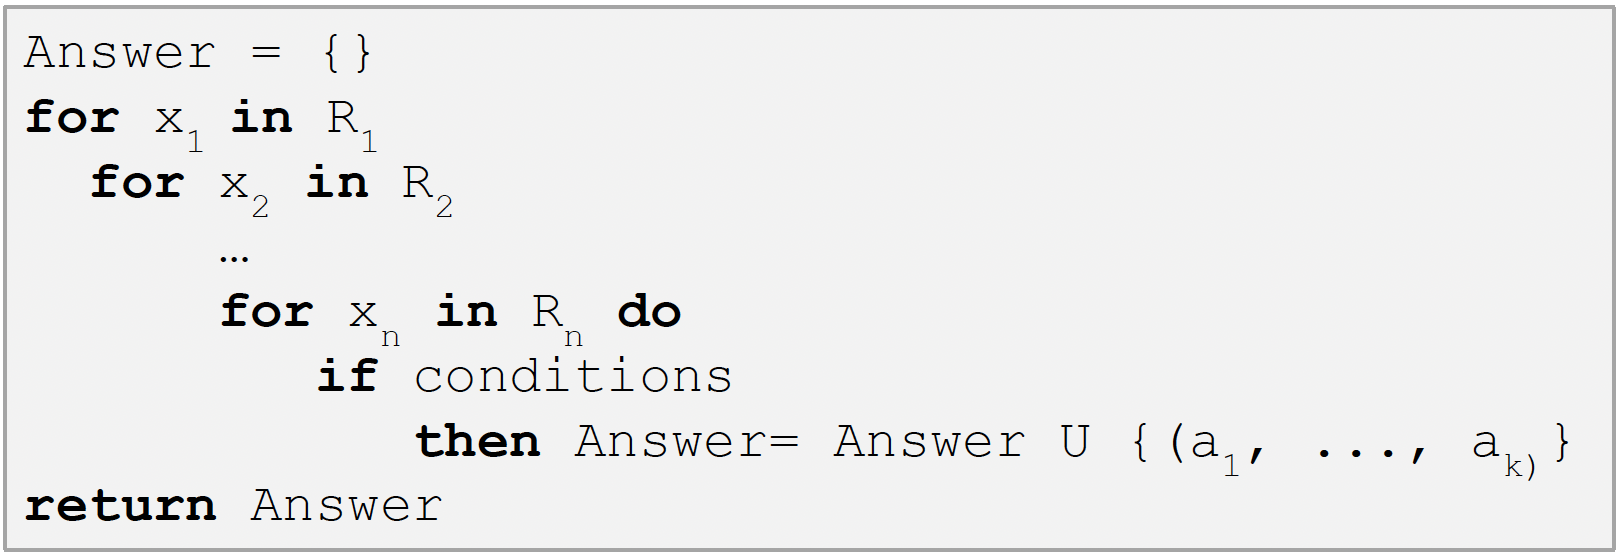
\includegraphics[width=10cm]{assets/nestedLoopsQuery.png}

The semantics of a SQL query can be given using nested loops \textit{or} by parallel assignments, which we can see below:

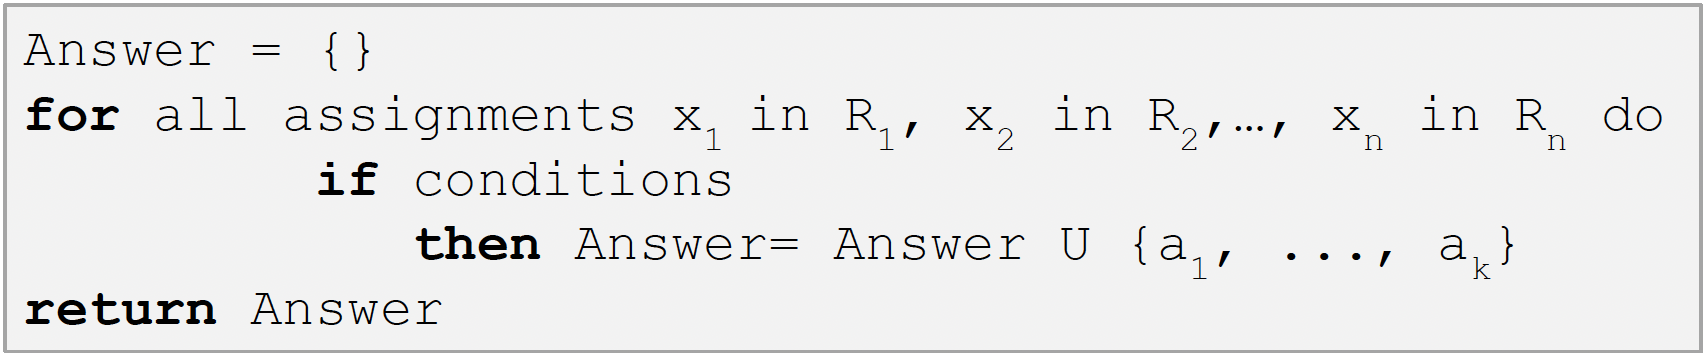
\includegraphics[width=10cm]{assets/parallelAssignmentQuery.png}

\textcolor{red}{Get a better sense of what parallel assignment means and how it differs from nested loops.}

Its important to understand how queries can be implemented so that we better understand when SQL does unintuitive things. These `SQLisms' occur especially often with empty tables or relations since an empty relation means the inner loop will not execute in the nested loops implementation -- leading to an empty query result.

This understanding also explains why the following query, which refers to two distinct relations \textit{R} and \textit{S} with a cardinality of 4 each, produces a table with a cardinality of 16. As we know, each record or tuple in the relation \textit{R} merges with every record or tuple in the relation \textit{S}:

\begin{tcolorbox}
    \begin{verbatim}
        SELECT *
        FROM R, S;
    \end{verbatim}
\end{tcolorbox}

\end{document}
